\documentclass[%
 reprint,
 amsmath,amssymb
 aps,
]{revtex4}

\usepackage{float}
\usepackage{subfig}
\usepackage{graphicx}% Include figure files
\usepackage{dcolumn}% Align table columns on decimal point
\usepackage{bm}% bold math
\usepackage{physics}
\setlength{}{}%
\usepackage{siunitx}
\usepackage[inline]{asymptote}
\usepackage{multirow}
\usepackage{tikz}
\usepackage{pgfplots, pgfplotstable}
\usepackage{hyperref}
\usepackage{natbib}
\usepackage{amsthm}
\usepackage{amssymb}
\usepackage{amsmath}
\usepackage{cancel}
\bibliographystyle{unsrtnat}
\pgfplotsset{compat=1.3}

\usepackage{pdfpages}

\theoremstyle{remark}
\newtheorem*{rem}{Remark}
\newtheorem*{note}{Note}
\newtheorem{claim}{Claim}

\begin{document}
\title{Traversable Wormholes in General Relativity: Can they exist?}
\author{QiLin Xue}
\maketitle
\tableofcontents
\vspace{4mm}

Wormholes are a common plot device used in several science fiction books and films, all including the iconic but wildly inaccurate ``bending paper in half and poking a hole with a pencil'' demonstration. This report will provide a rigorous introduction to the mathematics and physics behind wormholes. In particular, we will focus our attention on a certain type of traversable wormhole, developed by Michael Morris and Kip Thorne in 1988, as a realistic plot device for Carl Sagan's book \textit{Contact}\cite{Thorne}!
\vspace{2mm}

We will analyze the characteristics of this wormhole in more detail, and similar to Morris and Thorne's initial paper, show that this metric violates the null energy condition and demands for the existence of exotic matter. We build onto the original paper by showing that the average null energy condition is also broken, allowing us to quantify the amount of exotic matter needed for each wormhole geometry.
\section{Basic Metric}
In this report, we will consider inter-universe wormholes, which are wormholes that connect two universes. This allows symmetric arguments to be made, simplifying the mathematics. For intra-universe travel, one can imagine that the mouths of the wormhole are located far away such that the inter-universe wormhole metric is a good approximation. We can assume that in general, wormholes are static, nonrotating, and spherically symmetric, so the most general form is given by a variation of the Schwarzschild solution,\cite{Thorne}
\begin{equation}
    \dd{s}^2 = -e^{2\Phi(r)}\dd{t}^2 + \frac{\dd{r}^2}{1-b(r)/r} + r^2\left(\dd{\theta}^2 + \sin^2\theta\dd{\varphi}^2\right),
\end{equation} 
The two universes this wormhole connects intersects at $r=r_0$ and can be identified by having two coordinate charts $[r_0,\infty).$ The function $b(r)$ is known as the shape function and $\Phi_{\pm}(r)$ is the redshift function, where
\begin{align}
    \lim_{r\to\infty}b(r) = 2M
\end{align}
to retrieve the asymptotic limit. Note that this is not the most general metric. The redshift and shape function do not need to be the same in both universes. That is, time can run at different speeds\cite{Visser}. However, for simplicity and to allow this metric to be used for inter-universe wormholes, we will make these simplifying assumptions. The proper radial distance can be defined to be 
\begin{equation}
    \ell(r) = \pm \int_{r_0}^{r} \frac{\dd{r}}{\sqrt{1-b_{\pm}(r)/r}}.
\end{equation}
The throat of the wormhole is the minimum value of $r(\ell),$ which we denote as $r(0)=r_0.$ Since
\begin{equation}
    \frac{dr}{d\ell} = \pm \sqrt{1-\frac{b}{r}},
\end{equation}
we must have $b(r_0)=r_0,$ and $b(r) \le r.$ We can make the following claim,
\begin{claim}
    In some open neighborhood near the throat $(r_0,r_*),$ the following inequality holds:
    \begin{equation}
        b'(r) < \frac{b(r)}{r}.
        \label{eq:claim1}
    \end{equation}
    \begin{proof}
        The second derivative of $r$ with respect to the proper distance is 
        \begin{align}
            \frac{d^2r}{d\ell^2} &= \frac{dr}{d\ell}\frac{d}{dr}\left(\pm \sqrt{1-b/r}\right) \\ 
            &= \frac{1}{2r}\left(\frac{b(r)}{r}-b'(r)\right). \label{eq:2ndderivative}
        \end{align}
        Also recall that we can write 
        \begin{equation}
            r(\ell) = r_0 + \cancel{\frac{dr}{d\ell}\bigg|_{r=r_0}\ell} + \frac{1}{2!}\frac{d^2r}{d\ell^2}\bigg|_{r=r_0}\ell^2 + \mathcal{O}(\ell^3),
        \end{equation}
        Note that $r(\ell)$ is an increasing function, so $r''(\ell)$ must be positive in some neighbourhood near the throat. From \ref{eq:2ndderivative}, we see that this implies that $b'(r) < \frac{b(r)}{r}.$
        \vspace{2mm}
        
        It is important to recall that the increasing condition only implies that $r''(\ell)>0$ for $r\in (r_0,r_*),$ but the second derivative could still be zero at the point $r=r_0.$ This subtlety will be important later in claim 2.
    \end{proof}
\end{claim}
\subsection{Curvature}
We can compute the Einstein tensors. To make computations easier, we can consider a new coordinate system, defined by 
\begin{align}
    e_{\hat{t}} &= e^{-\Phi}e_t \\ 
    e_{\hat{r}} &= (1-b/r)^{1/2}e_r \\ 
    e_{\hat{\theta}} &= \frac{1}{r}e_{\theta} \\
    e_{\hat{\varphi}} &= \frac{1}{r\sin\theta}e_{\varphi},
\end{align}
such that the metric in this basis takes on the standard Minkowski metric, $\eta_{\hat{\mu}\hat{\nu}} = e_{\hat{\mu}}e_{\hat{\nu}}.$ It can then be computed (as done in the Appendix), that 
\begin{align}
    G_{\hat{t}\hat{t}} &= \frac{b'(r)}{r^2} \label{eq:G_tt} \\ 
    G_{\hat{r}\hat{r}} &= -\frac{b(r)}{r^3} + \frac{2}{r}\left(1-\frac{b(r)}{r}\right)\Phi'(r) \\ 
    G_{\hat{\theta}\hat{\theta}} = G_{\hat{\varphi}\hat{\varphi}} &= \frac{1}{2r^3}\left\{[1+r\Phi'(r)]\left[b(r)-rb'(r)+2r^2\left(1-\frac{b(r)}{r}\right)\Phi'(r)\right]\right\} + \left(1-\frac{b(r)}{r}\right)\Phi''(r).
\end{align}
At the throat $r=r_0,$ these become 
\begin{align}
    G_{\hat{t}\hat{t}}\bigg|_{r_0} &= \frac{b'(r_0)}{r_0^2} \\ 
    G_{\hat{r}\hat{r}}\bigg|_{r_0} &= -\frac{1}{r_0^2} \label{eq:G_rr0}\\ 
    G_{\hat{\theta}\hat{\theta}}\bigg|_{r_0} = G_{\hat{\varphi}\hat{\varphi}}\bigg|_{r_0} &= \frac{1}{2r_0^2}(1+r_0\Phi'(r_0))(1+b'(r_0)).
\end{align}
Let the stress energy tensor be $T=\text{diag}(\rho,-\tau,p,p),$ where $\tau = -p_r$ is the radial \textit{tension}. Einstein's equation $G_{\mu \nu}=8\pi T_{\mu\nu}$ gives, for equation \ref{eq:G_tt},
\begin{equation}
    b'(r) = 8\pi \rho r^2,
    \label{eq:b-v-r}
\end{equation}
and integrating, we obtain
\begin{equation}
    b(r) = b(r_0) + 2\int_{r_0}^{r} 4\pi \rho r^2 \dd{r}.
\end{equation}
We can identify this as a mass term, allowing us to define $b(r)=2m(r),$ with 
\begin{equation}
    m(r) = \frac{r_0}{2} + \int_{r_0}^r 4\pi \rho r^2 \dd{r}.
\end{equation}
Notice that this definition was made such that it agrees with the definition of mass in the Schwarzschild solution when $r_0 = 0.$ Let $\rho_,\tau_0,p_0$ be the corresponding stress energy coefficients at $r=r_0.$ We can write the following relationship,
\begin{claim}
    For some open neighbourhood near the throat $(r_0,r_*),$ the following inequality holds:
    \begin{equation}
        \rho_0 \le \tau_0.
    \end{equation}
    \begin{proof}
        Using claim 1 with equation \ref{eq:b-v-r} gives 
        \begin{equation}
            8\pi \rho r^2 < \frac{2m(r)}{r},
        \end{equation}
        where the substitution $b(r)=2m(r)$ was made. Rearranging for $\rho_0,$ we have 
        \begin{equation}
            \rho_0 \le \frac{1}{8\pi r_0^2}.
        \end{equation}
        Note that the inequality is weaker now because we are looking at the point $r=r_0$ and not the open neighborhood $(r_0,r_*).$ Equation \ref{eq:G_rr0} along with Einstein's equation gives 
        \begin{equation}
            \tau_0 = \frac{1}{8\pi r_0^2}.
        \end{equation}
        Combining these together gives the desired inequality.
    \end{proof}
    This is an important result which we will later show gives rise to energy condition violations, motivating the need for exotic matter.
\end{claim}

% We can obtain a few important properties of this metric.
% \begin{proof}
    % \begin{equation}
    %     \frac{dr}{d\ell} = \pm \sqrt{1-\frac{b}{r}},
    % \end{equation}
    % so there must be som 

    % so the second derivative is 
    % \begin{align}
    %     \frac{d^2r}{d\ell^2} = \frac{dr}{d\ell}\frac{d}{dr}\left(\pm \sqrt{1-b/r}\right) = \frac{1}{2r}\left(\frac{b(r)}{r}-b'(r)\right).
    % \end{align}
% \end{proof}
\subsection{Motivation}
The motivation for why the Schwarzschild metric might possibly be related to inter-universe travel is subtle, and neglected by many authors such as Thorne, Visser, and Lobo, other than a brief mention\cite{Thorne}\cite{Visser}\cite{Lobo}. We work out the details in this section, following the work done by Ludwig Flamm in 1916, who at the time, did not make the connection to wormholes\cite{Gibbons}.

Recall that the universe can be described by a 3-sphere embedded in $\mathbb{R}^4,$ such that the spatial part of its metric is given by 
\begin{equation}
    \dd{\sigma}^2 = R_0^2\left(\dd{\psi}^2 + \sin^2\psi\dd{\varphi}^2+\sin^2\psi\sin^2\theta\dd{\theta}^2\right).
\end{equation} 
Taking the equatorial slice $\theta=\frac{\pi}{2},$ it reduces down to the metric for a 2-sphere,
\begin{equation}
    \dd{\sigma}^2 = R_0^2\left(\dd{\psi}^2 + \sin^2\psi\dd{\varphi}^2\right).
\end{equation}
This is the metric for a surface generated by a curve, in this case, a circle. Let the coordinate $z$ point in the direction of the axis of rotation, and let $\psi \in [0,2\pi)$ be the angle spanning the circle, such that the arc-length of this circle is given by $R_0\psi.$ Let the coordinate $R$ point in the direction perpendicular to $z,$ in the plane of the circle. Then, we have 
\begin{equation}
    \frac{dz}{dr} = \tan\psi. \label{eq:dzdr}
\end{equation}
In this specific example, we have $\sin\psi = \frac{R}{R_0}$ so equation \ref{eq:dzdr} gives 
\begin{equation}
    \frac{dz}{dr} = \pm \frac{R}{\sqrt{1-R^2/R_0^2}},
\end{equation}
and integrating gives 
\begin{equation}
    z^2 = R_0^2 - R^2,
\end{equation}
which is the equation of a circle, as expected. We can apply this technique to the Schwarzschild metric, where the corresponding spatial metric is 
\begin{equation}
    \dd{\sigma}^2 = \frac{1}{1-2M/r}+r^2\dd{\varphi}^2.
\end{equation}
Consider the substitution $\cos^2\psi = 1 - \frac{2M}{r}.$ We can compute,
\begin{equation}
    -\sin\psi\cos\psi \dd{\psi} = \frac{2M}{r^2}\dd{r},
\end{equation}
which yields 
\begin{equation}
    \dd{r}^2 = \left(1-\frac{2M}{r}\right) \cdot \frac{r^2}{2M}\dd{\psi}^2
\end{equation}
Using this, we have,
\begin{align}
    \dd\sigma^2 &= \frac{\dd{r}^2}{1-2M/r}+r^2\dd{\varphi}^2 \\ 
    &= \frac{r^3}{2M} \dd{\psi}^2 + r^2\dd{\varphi}^2 \\ 
    &= \frac{r^3}{2M}\left(\dd{\psi}^2 + \frac{2M}{r}\dd{\varphi}^2\right) \\ 
    &= \frac{r^3}{2M}\left(\dd{\psi}^2 + \sin^2\psi\dd{\varphi}^2\right).
\end{align}
Which is in the same form as the metric of a 2-sphere. Solving the differential equation 
\begin{equation}
    \frac{d\psi}{dr} = \sqrt{\frac{2M}{r-2M}}
\end{equation} 
gives
\begin{equation}
    z^2 = 8M(r-2M),
\end{equation}
which is plotted in the figure below, for the case $M=1.$
\begin{center}
    \begin{tikzpicture}[scale=1]
    \begin{axis}[
    legend pos=outer north east,
    axis lines = middle,
    xlabel = $r$,
    ylabel = $z$,
    variable = t,
    trig format plots = rad,
    xmin = 0,
    ]
    \addplot [
        domain=2:10,
        samples=100,
        color=blue,
        ]
        {sqrt(8*x-16)};
        \addplot [
            domain=2:10,
            samples=100,
            color=blue,
            ]
            {-sqrt(8*x-16)};
        \end{axis}
    \end{tikzpicture}

\end{center}
Rotating this curve about the $z$-axis then generates the standard wormhole embedding diagram, i.e. it encloses two asymptotically flat regions of space, and is visualized in the diagram below. The curve in black depicts the generating curve this coordinate transformation produces.
\begin{center}
    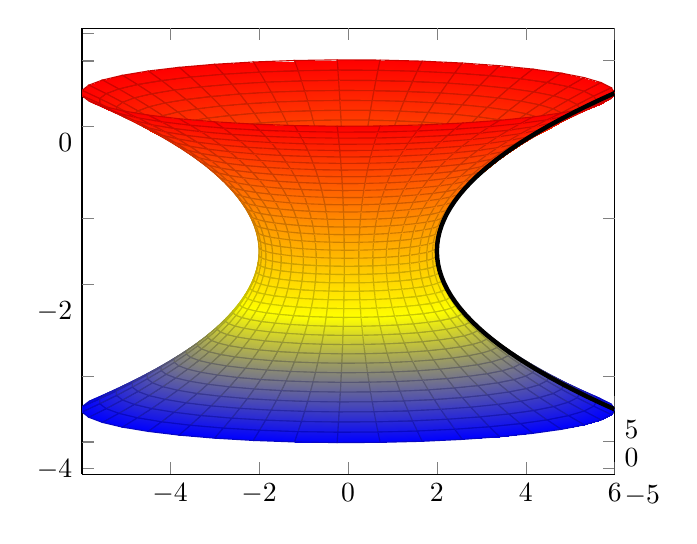
\begin{tikzpicture}
        \begin{axis}[view={0}{10}]
         \addplot3[surf,
         shader = faceted interp,
         samples=40,
         domain=-2:2,y domain=0:2*pi,
         z buffer=sort]
         ({(x^2+2) * cos(deg(y))}, {(x^2+2)* sin(deg(y))}, {x-2});
         \addplot3+[no markers,
         samples=51,
         samples y=0,
         domain=-2:2,
         variable=\t,
         color=black,
         line width = 0.7pt,
         ultra thick
         ]
         ({(\t^2+2) * cos(deg(0))}, {(\t^2+2)* sin(deg(0))}, {\t-2});
        \end{axis}
       \end{tikzpicture}   
\end{center}
\section{Exotic Matter}
Energy conditions are used in general relativity to represent requirements for the energy density to be positive. The weak energy condition and null energy condition both require that\cite{Wald}
\begin{equation}
    \rho + p_i \ge 0
\end{equation}
for $i=1,2,3.$ However, recall that in the region $(r_0,r_*),$ the inequality
\begin{equation}
    \rho + (-\tau) < 0
\end{equation}
holds and therefore violates both the weak energy and null energy condition. This is expected, since if a beam of laser was shot through the wormhole, its cross-sectional area will first decrease before increasing, and this behavior can only be caused by gravitational repulsion, which requires exotic matter\cite{Thorne}. Classically, particles obey the weak energy condition, but in quantum field theory, there are examples where this energy condition is broken. In fact, all energy conditions used in general relativity are broken in quantum field theory\cite{Lobo}. Quantum field theory is beyond the scope of this report, so the discussion on exotic matter will end here.
\subsection{Average Null Energy Condition}
Instead of requiring that the energy density be positive everywhere, we can instead require that the average energy density be positive, such that if we integrate over a null curve $\Gamma,$ we have 
\begin{align}
    I_{\Gamma} = \int_{\Gamma} (\rho - \tau) \xi^2 \dd{\lambda} \ge 0,
\end{align}
where $\xi$ is a radial null geodesic. Because the geodesic is radial, we can parametrize the curve using the proper distance $\ell$ such that 
\begin{align}
    \dd{t} = \sqrt{\frac{g_{rr}}{g_{tt}}}\dd{r} = \frac{e^{-\Phi(r)}}{\sqrt{1-b(r)/r}}\dd{r} = e^{-\Phi(r)}\dd{\ell}.
\end{align}
Since $\frac{\dd{\lambda}}{\dd{t}} = g_{tt} = e^{2\Phi(r)},$ we can rewrite 
\begin{align}
    I_{\Gamma} &= \int_{-\infty}^{\infty} (\rho - \tau)e^{-\Phi}\dd{\ell} \\ 
    &= -\frac{1}{4\pi}\int_{r_0}^{\infty}\frac{1}{r^2}e^{-\Phi}\sqrt{1 - \frac{b(r)}{r}}\dd{r},
\end{align}
where the second line is derived by applying the Einstein field equations to write formulas for $\rho$ and $\tau,$ then integrating by parts\cite{Visser}. Note that the integrand will always be positive, so $I_{\Gamma} < 0,$ violating the average null energy condition.
\vspace{2mm}

The quantity $I_{\Gamma}$ allows for us to quantify how much exotic matter is needed for a certain wormhole geometry. In the later section, we will consider a few specific wormhole geometries that allows traversability and compute this integral. While it is impossible to satisfy the average null energy condition, we can do our best to minimize the amount of exotic matter needed.

\section{Traversability}
We will use a working definition of traversable wormholes to be one such that a person can traverse through it without dying and in a reasonable amount of time. This definition is different from some authors such as Matt Visser, who define it to be any wormhole that is macroscopic and exists for a finite amount of time. In this section, we will see that such a wormhole is indeed possible to construct, given that we have access to exotic matter. Consider a trajectory that starts at proper radial distance $\ell = -\ell_0$ and $\ell = +\ell_0$ and the velocity vector is always radial.

The proper time must be 
\begin{align}
    \int_{-\ell_1}^{\ell_1} \frac{1}{v\gamma}\dd{\ell} < \text{ 1 year},
\end{align}
where $v$ is the speed as measured by a stationary observer. The $1$ year requirement is completely arbitrary, but was given to be in agreement with Morris and Thorne\cite{Thorne}. To not die, the traveler must experience minimal tidal forces. We wish to work in the coordinates of the traveler, which we can do with the Lorentz transformation,
\begin{align}
    e_{\hat{0}} = U &= \gamma e_{\hat{t}} -\gamma v e_{\hat{r}} \\
    e_{\hat{1}} &= -\gamma v e_{\hat{t}} + \gamma e_{\hat{r}} \\
    e_{\hat{2}} &= e_{\hat{\theta}} \\
    e_{\hat{3}} &= e_{\hat{\varphi}},
\end{align}
where $U^{\mu}=(1,0,0,0)$ is the 4-velocity in this new frame.
The tidal force is given by 
\begin{equation}
    (\Delta a)^{\mu} = -R^{\mu}{}_{\alpha\nu\beta}U^{\alpha}(\Delta \xi)^{\nu}U^{\beta}= -R^{\mu}{}_{\hat{0}\nu\hat{0}}U^{\hat{0}}(\Delta \xi)^{\nu}U^{\hat{0}},
\end{equation}
where $R^{\mu}{}_{\hat{0}\nu\hat{0}}$ is sometimes known as the tidal tensor. Tensor transformation laws give us 
\begin{align}
    R^{\hat{1}}{}_{\hat{0}\hat{1}\hat{0}} &= \gamma^4 R^{\hat{r}}{}_{\hat{t}\hat{r}\hat{t}} \\
    R^{\hat{2}}{}_{\hat{0}\hat{2}\hat{0}} = R^{\hat{3}}{}_{\hat{0}\hat{3}\hat{0}} &= \gamma^2 R^{\hat{\theta}}{}_{\hat{t}\hat{\theta}\hat{t}}  + \gamma^2v^2R^{\hat{\varphi}}{}_{\hat{t}\hat{\varphi}\hat{t}}.
\end{align}
Note that in Thorne's original paper, they omitted the $\gamma^4$ term, but as we shall soon see, minimizing the tidal force implies that we must demand $v \ll 1$ so $\gamma \sim 1$ and we can ignore it\cite{Thorne}. We can compute,
\begin{align}
    (\Delta a)^{\hat{0}} = -R^{\hat{0}}{}_{\hat{0}\nu\hat{0}}U^{\hat{0}}(\Delta \xi)^{\nu}U^{\hat{0}}.
\end{align}
This is zero since as shown in the Appendix, no nonzero curvature tensors have more than two indices being a $t$, once we transform make to the observer's frame. Instead, we note that 
\begin{align}
    (\Delta a)^{\hat{1}} &= -R^{\hat{1}}{}_{\hat{0}\nu \hat{0}}U^{\hat{0}}(\Delta \xi)^{\nu}U^{\hat{0}}, \\
    (\Delta a)^{\hat{2}} &= -R^{\hat{2}}{}_{\hat{0}\nu \hat{0}}U^{\hat{0}}(\Delta \xi)^{\nu}U^{\hat{0}},
\end{align}
where after applying the relevant tensor transformation laws, give us
\begin{align}
    \left|\left(1-\frac{b(r)}{r}\right)\left\{-\Phi''-(\Phi')^2\right\}+\frac{1}{2r^2}(b'(r)r-b(r))\Phi'\right| \le \frac{g}{L} \\ 
    \frac{\gamma^2}{r^2}\left|(r-b(r))\Phi'+\frac{v^2}{2}\left(b'(r) - \frac{b(r)}{r}\right)\right| \le \frac{g}{L},
\end{align}
where $L=|\Delta \xi|$ is the maximum distance between two points on the human body, and $g$ is the maximum tidal acceleration. The first inequality constrains the redshift function and the second inequality constrains the speed at which the traveler is moving at. Typically, the behavior at the throat of the wormhole is characteristic of the overall behaviour since forces tend to be maximal there. We obtain,
\begin{align}
    |\Phi'| \le \frac{2gr_0}{(1-b'(r))L} \\ 
    \gamma^2v^2 \le \frac{2gr_0^2}{(1-b'(r))L}.
\end{align} 
The greater the throat $r_0$ is, the greater the freedom for the redshift function. Similarly, we get more freedom if $b'(r)$ approaches $1.$ We will examine a few simple solutions.
\subsection{Constant Redshift}
If the redshift is constant, i.e. $\Phi'=0$ then we can obtain for all values of $r,$
\begin{equation}
    \frac{\gamma^2v^2}{2r^2}\left|b'(r)-\frac{b(r)}{r}\right| \le \frac{g}{L}.
\end{equation} 
Unlike in general, i.e. in the gravitational field of a massive object, there are no tidal forces when the traveler is stationary $v=0.$ Note that all our curvature terms depend only on $\Phi'$ and not $\Phi,$ so to make things simpler, this gives the same results as choosing $\Phi=0,$ which some authors have chosen to do instead\cite{Lobo}. It is also why this form of solution is sometimes known as the \textit{zero tidal solution.} We can choose the shape function to satisfy the conditions of the wormhole described in the first section. With this new metric, one possible shape function is given by
\begin{equation}
    b(r) = \sqrt{b_0r}.
\end{equation}
Thorne shows that the inequalities we derived above imply that $b=10\text{ m},v = 60\text{ m/s}$ and $\Delta \tau = 1 \text{ hour}$ satisfy the required inequalities\cite{Thorne}. However, note that the Einstein tensors take on the simpler form,
\begin{align}
    G_{\hat{t}\hat{t}} &= \frac{b'}{r^2} = 8\pi \rho \\ 
    G_{\hat{r}\hat{r}} &= -\frac{b}{r^3} = -8\pi \tau \\ 
    G_{\hat{\theta}\hat{\theta}} = G_{\hat{\varphi}\hat{\varphi}} &= \frac{1}{2r^3}(b-b'r) = 8\pi p,
\end{align}
allowing us to directly compute
\begin{equation}
    \rho - \tau = -2p,
\end{equation}
so the weak energy condition will be violated everywhere, and not just localized to a specific spot\cite{Visser}. This is extremely troubling, and other shape functions will exhibit this same behavior. This suggests that while constant redshift may be a good model for traversability, it is very unlikely to exist if we wish to minimize the amount of exotic matter needed. Namely, the average null energy integral gives 
\begin{align}
    I_{\Gamma} &= -\frac{1}{4\pi} \int_{r_0}^{\infty} \frac{1}{r^2}\sqrt{1-\frac{\sqrt{b_0r}}{r}}\dd{r} \\ 
    & -\frac{2}{15\pi r_0},
\end{align}
where we recall that $b_0=b(r_0)=r_0.$ Therefore, the amount of exotic energy we need scales by $\frac{1}{r_0}$ This makes sense, as a larger wormhole would require more exotic energy to keep it together.

\subsection{Zero Density}
Similarly, we can consider choosing the shape function to be a constant $b(r)=r_0$ instead, and allow us to choose an appropriate redshift function. Note that for all redshift functions, we have $G_{\hat{\tau}\hat{\tau}}=0$ so we have,
\begin{equation}
    \rho - \tau = -\frac{r_0}{8\pi r^3} + \frac{1}{4\pi}\left(1-\frac{r_0}{r}\right)\frac{\Phi'}{r}
\end{equation}
which comes from the Einstein equations. One possible redshift function we can choose is one that in the limit, allows us to obtain the standard Schwarzschild metric, i.e. choose $\Phi$ such that
\begin{align}
    \dd{s}^2 = -\left(1-\frac{r_0}{r}+\frac{\epsilon}{r^2}\right)\dd{t}^2 + \frac{\dd{r}^2}{1-\frac{r_0}{r}} + r^2\left[\dd{\theta}^2 + \sin^2\theta\dd{\varphi}^2\right]
\end{align}
The average null energy integral can be computed by recognizing that 
\begin{equation}
    e^{-\Phi(r)} = \left(1-\frac{r_0}{r}+\frac{\epsilon}{r^2}\right)^{-1/2} = r\sqrt{\frac{1}{r^2-r_0r+\epsilon}},
\end{equation}
such that 
\begin{align}
    I_{\Gamma} = -\frac{1}{4\pi}\int_{r_0}^{\infty} \frac{1}{r}\sqrt{\frac{1}{r^2-r_0r+\epsilon}} \sqrt{1-\frac{r_0}{r}}\dd{r}.
\end{align}
The integrand is a monotonically decreasing function of $\epsilon$ for all values of $r\in (r_0,\infty),$ so we can create a lower bound by setting $\epsilon = 0.$ After simplifying, we get,
\begin{align}
    &I_{\Gamma} > -\frac{1}{4\pi}\int_{r_0}^{\infty}\frac{1}{r^2}\dd{r} \\ 
    \implies & -\frac{1}{4\pi r_0} < I_{\Gamma} < 0,
\end{align}
so the amount of exotic energy we need is bounded by $1/r_0,$ which has the same behavior as the constant redshift black hole. The only difference is that in this metric, the exotic matter is contained in only a small section of the wormhole. Particularly, the regions with high radial tension, and thus violate the weak energy condition has a width of around the order $r \sim \sqrt{\epsilon}$\cite{Visser}. Therefore, if $\epsilon = 0,$ no energy conditions will be violated at or near $r=r_0.$ However, $\epsilon = 0$ returns us the standard Schwarzschild metric, where $r=r_0$ is the event horizon. Therefore, we see that by adding a small correction term, we are able to turn what was initially the event horizon into the throat of a wormhole connecting two universes.

% This implies that $\Delta a$ must also only spatial components because 
% \begin{align}
%     \left(\Delta a\right)^{\hat{\tau}} &= -R^{\hat{\tau}}{}_{\alpha \nu\beta}V^{\alpha}(\Delta \xi)^{\nu}V^{\beta} \\ 
%     &= -R^{\hat{\nu}}{}_{\hat{\beta}\hat{\tau}\alpha}V^{\alpha}(\Delta \xi)^{\nu}V^{\beta}
% \end{align}

\bibliographystyle{unsrt}%Used BibTeX style is unsrt
\bibliography{sample}

\newpage
\section{Appendix}
The code was heavily inspired by James B. Hartle's online \href{ @misc{mathematica, url={http://web.physics.ucsb.edu/~gravitybook/mathematica.html}, journal={Mathematica}} }{repository}. 
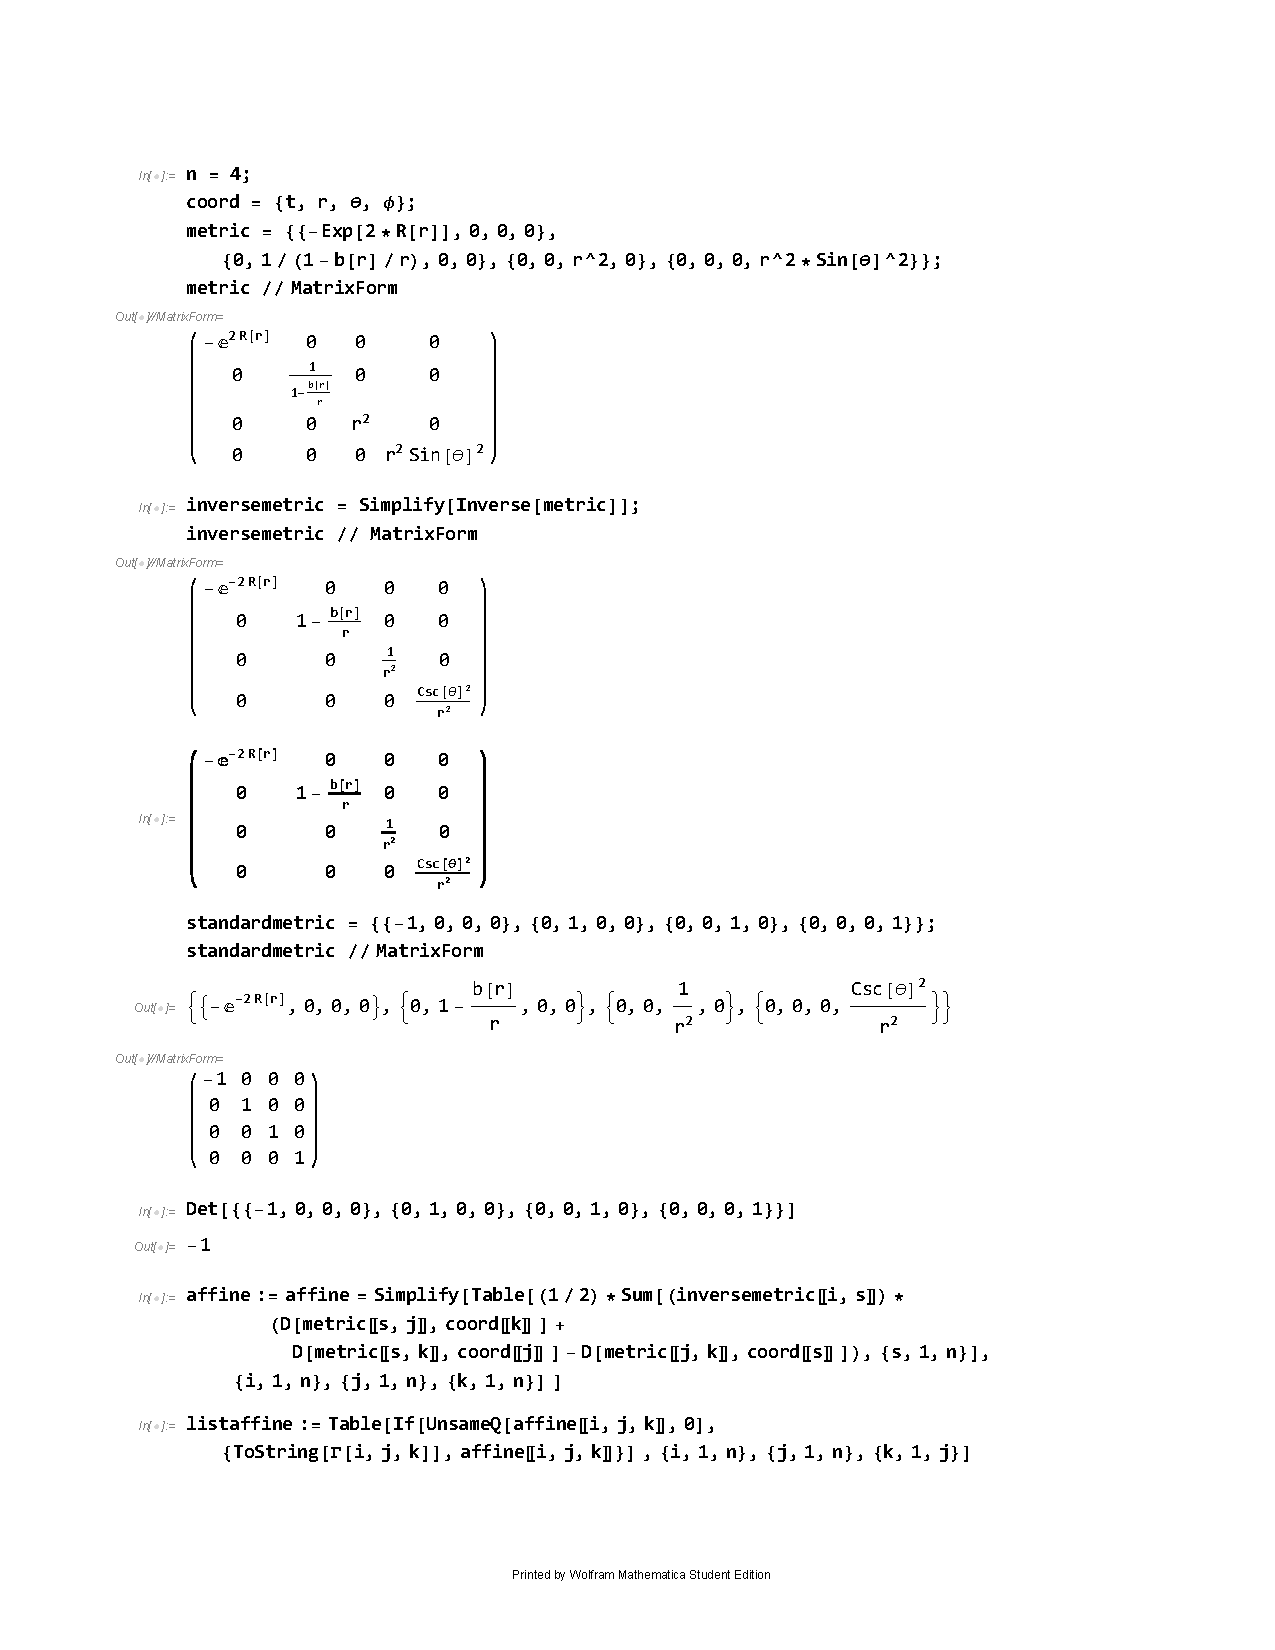
\includepdf[pages=-]{wormhole.pdf}
\end{document}
